\chapter{Estimations of a CI for the \texorpdfstring{\Xibz-\Lb}{Ξb-Λb} Ratio}
\label{chap:apdx_brxiblb}
The fit parameter $f_s$ of the model that we established in Sec.~\ref{sec:fit_model} can be used to estimate the branching fraction of the \Xibz and \Lb baryon into \Dz\Lz up to corrections due to the different \bquark-fragmentations:
\begin{equation}
    \label{eq:apdx_brxiblb_fs}
    \frac{f_{\Xibz}}{f_{\Lb}} \times \frac{\BR(\decay{\Xibz}{\Dz\Lz})}{\BR(\decay{\Lb}{\Dz\Lz})} = \frac{1 - f_s}{f_s} =: f(\Xibz/\Lb) \,,
\end{equation}
where $f_{\Lb} / f_{\Xibz}$ is the ratio of the fragmentation fractions of $\bquark$-quarks into \Lb and \Xibz baryons.

Two frequentist confidence intervals (CI) according to Ref.~\cite{NeymanPearson} are calculated by drawing random events from to the fitted \gls{pdf} where all parameters are fixed, except for $f_1$ and $f_s$.
While $\hat f(\Xibz/\Lb)$ is varied on the interval $[0.0 \, \ldots \, 0.6]$, the value of $f_1$ is corrected such that the ratio of the \Lb signal and the combinatorial background $f_s (1 - f_1) / f_1$ stays constant.
For each value of $\hat f(\Xibz/\Lb)$, 400 fits are performed.
Each of these fits yields a value for $f_s$ which is used to calculate $f_\text{obs}(\Xibz/\Lb)$, according to Eq.~\eqref{eq:apdx_brxiblb_fs}.
CIs are estimated by finding intervals in $\hat f(\Xibz/\Lb)$ such that, according to the pseudo-experiment, for each value of $\hat f(\Xibz/\Lb)$ within this interval, intervals with a given coverage in $f_\text{obs}(\Xibz/\Lb)$ include the value that was found with the fit to recorded data.
In total, we evaluate 25 different $\hat f(\Xibz/\Lb)$ values and smooth the estimated boundaries with linear functions.

Two different methods of finding the intervals in $f_\text{obs}(\Xibz/\Lb)$ are used:
In Fig.~\ref{fig:apdx_brxiblb_freqci_central} we show the result of the \textit{central} method where the 400 different outcomes are partitioned at the 16\,\% (5\,\%) and 84\,\% (95\,\%) percentiles, \ie{}, the central interval corresponds to 68\,\% (90\,\%) CL.
We note that this method of constructing two-sided intervals implicitly gives the one-sided 84\,\% (95\,\%) CL upper limit, too.
\begin{figure}[htbp]
    \centering
    \begin{subfigure}{.49\textwidth}
        \centering
        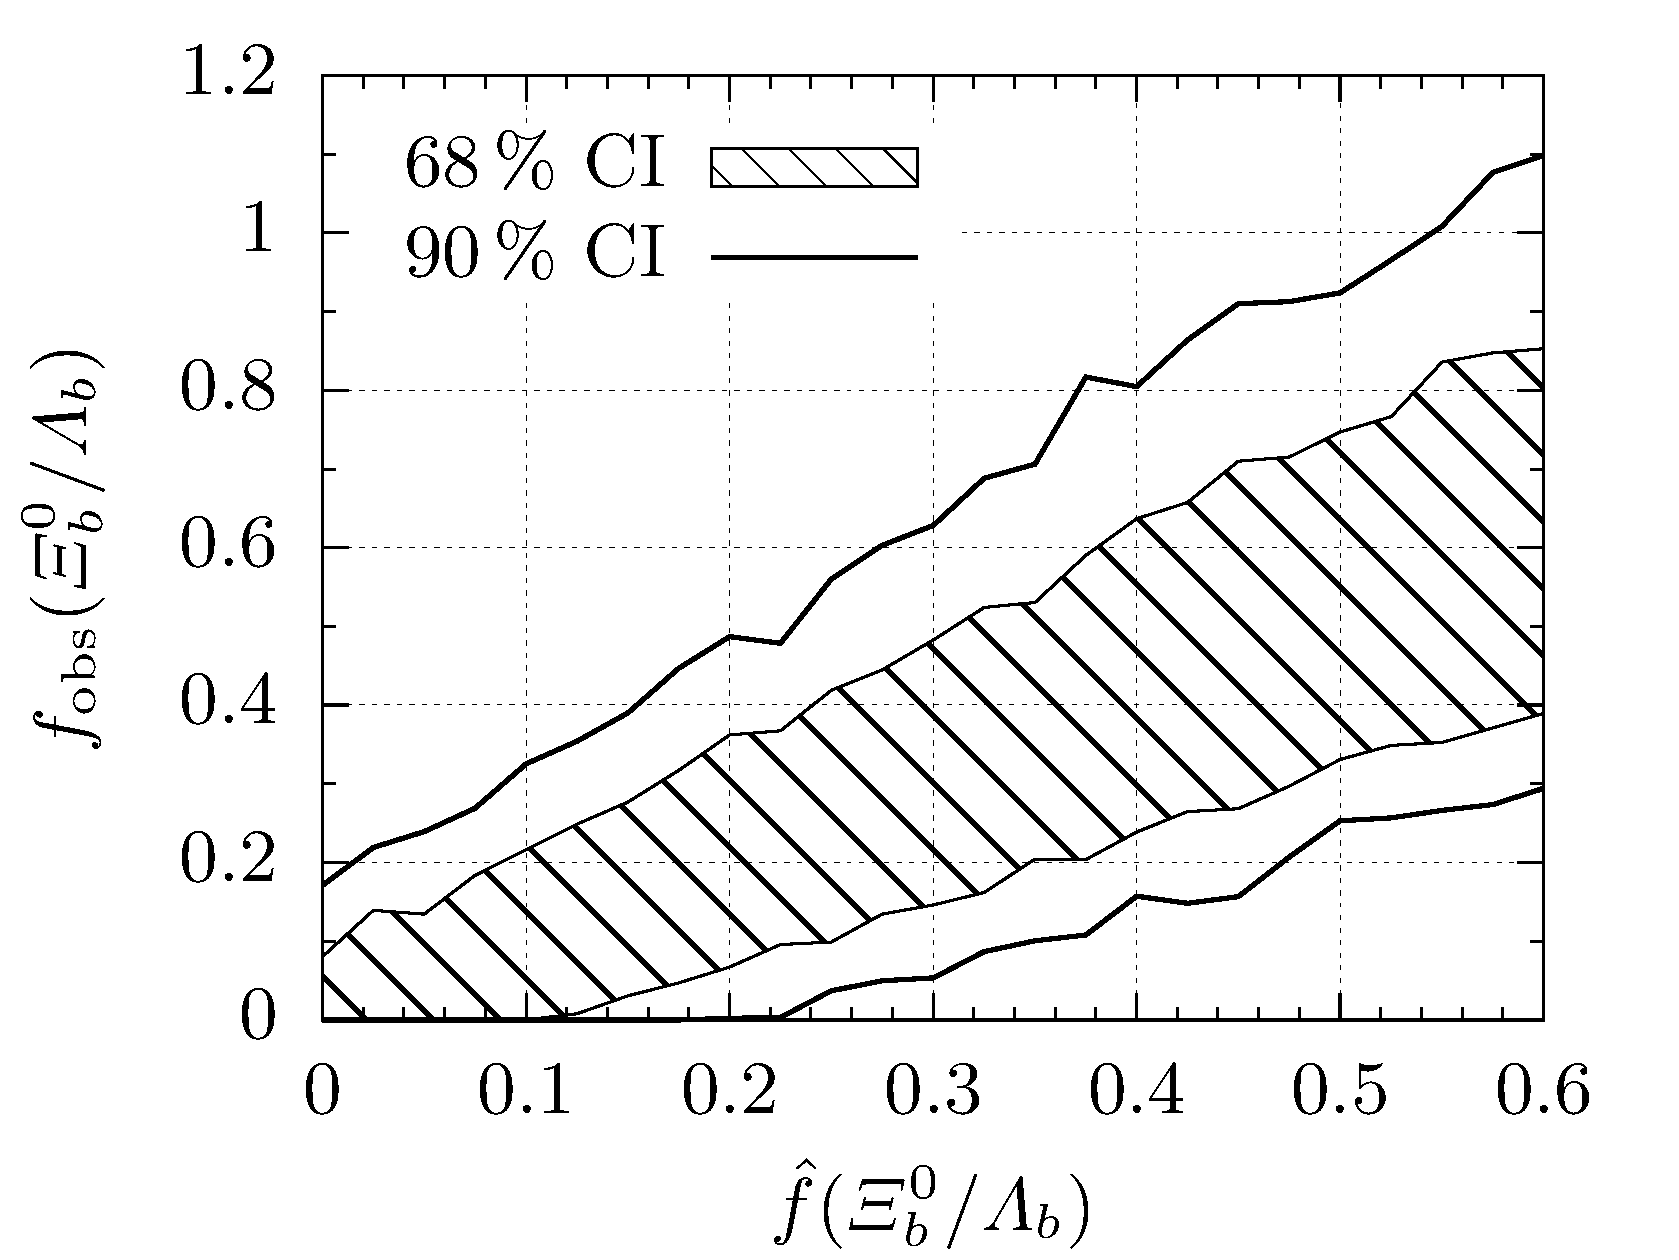
\includegraphics[scale=1.]{br/freqci.png}
    \end{subfigure}
    \begin{subfigure}{.49\textwidth}
        \centering
        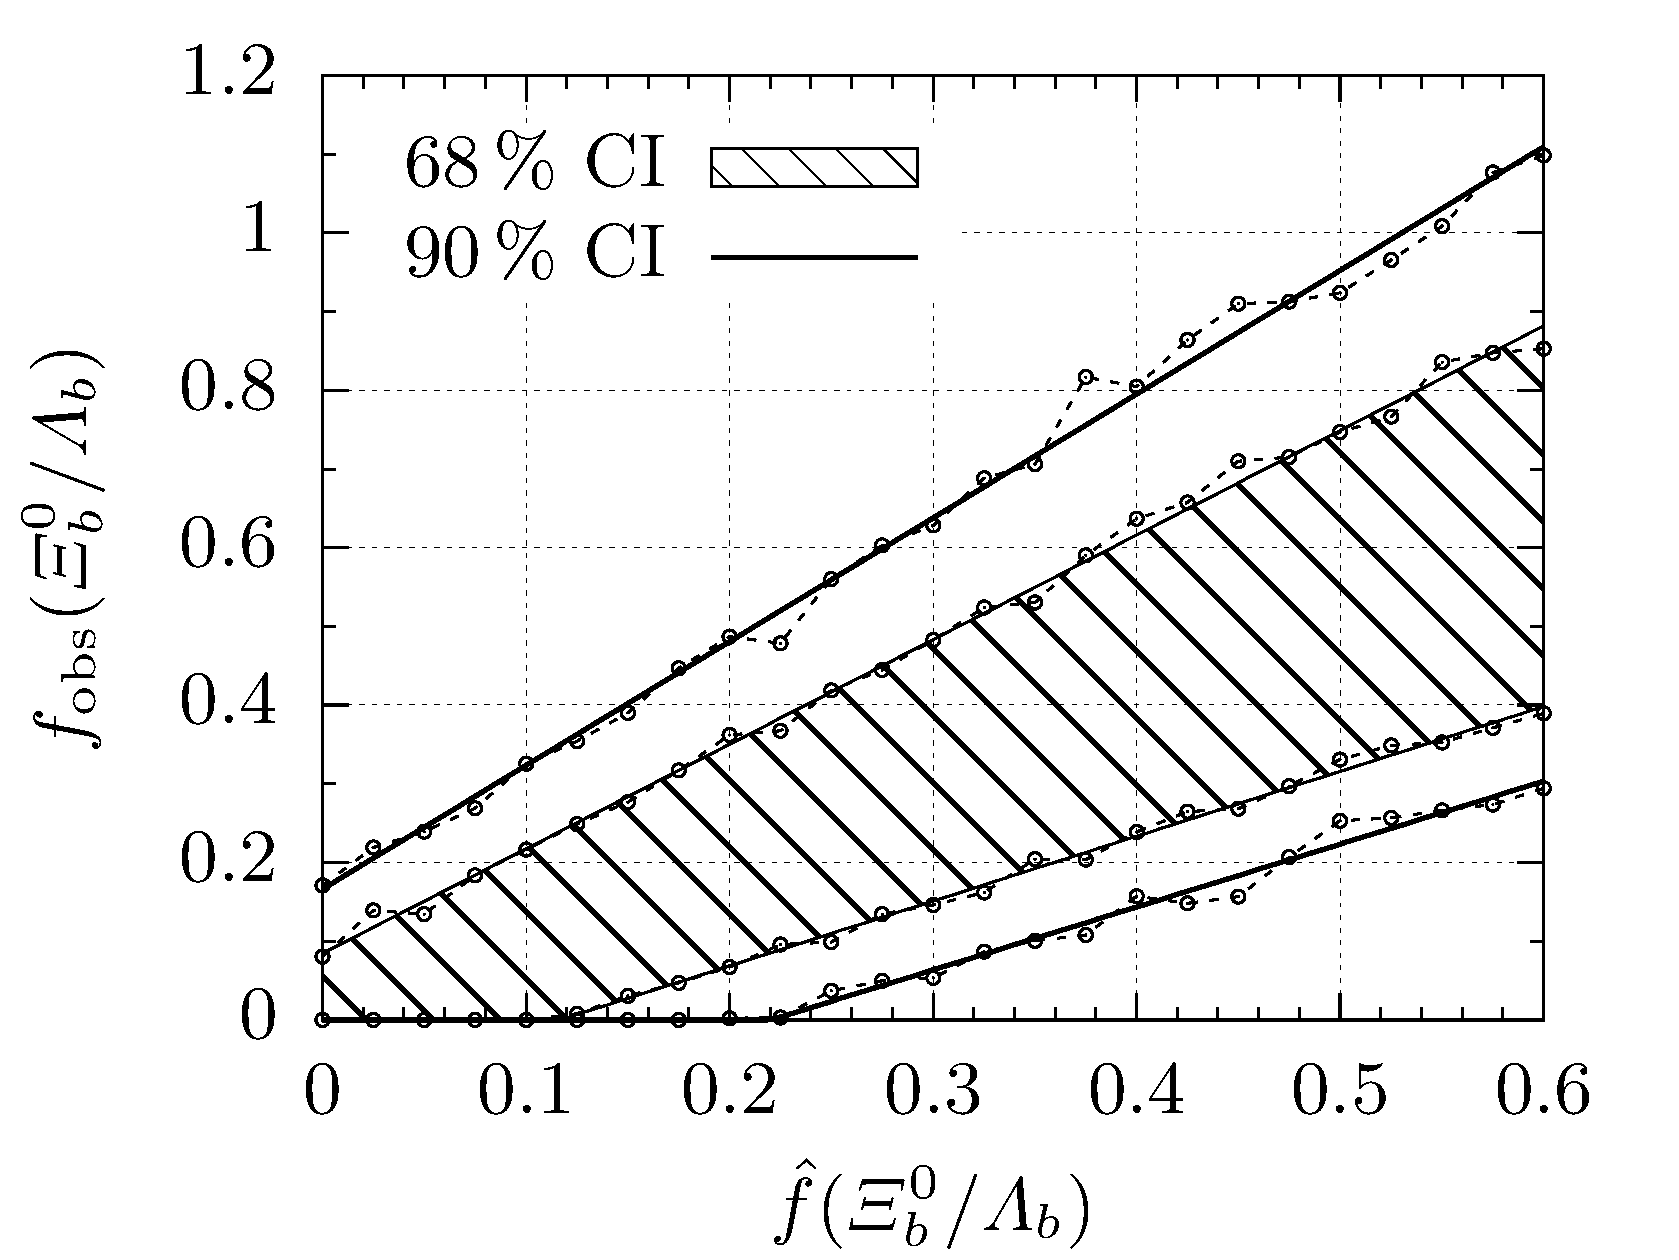
\includegraphics[scale=1.]{br/freqci-fit.png}
    \end{subfigure}
    \caption{Frequentist CIs using the \textit{central} method. Interval boundaries are estimated by percentiles in $f_\text{obs}(\Xibz/\Lb)$ at 25 different $\hat f(\Xibz/\Lb)$ positions. The boundaries (left) are smoothed with linear functions (right).}
    \label{fig:apdx_brxiblb_freqci_central}
\end{figure}

In Fig.~\ref{fig:apdx_brxiblb_freqci_shortest} we show the result of the \textit{shortest} method where for each value of $\hat f(\Xibz/\Lb)$ the shortest interval in $f_\text{obs}(\Xibz/\Lb)$ with a 68\,\% and 90\,\% coverage is estimated.
The output of this method is noisier and does not allow an extraction of upper limits.
\begin{figure}[htbp]
    \centering
    \begin{subfigure}{.49\textwidth}
        \centering
        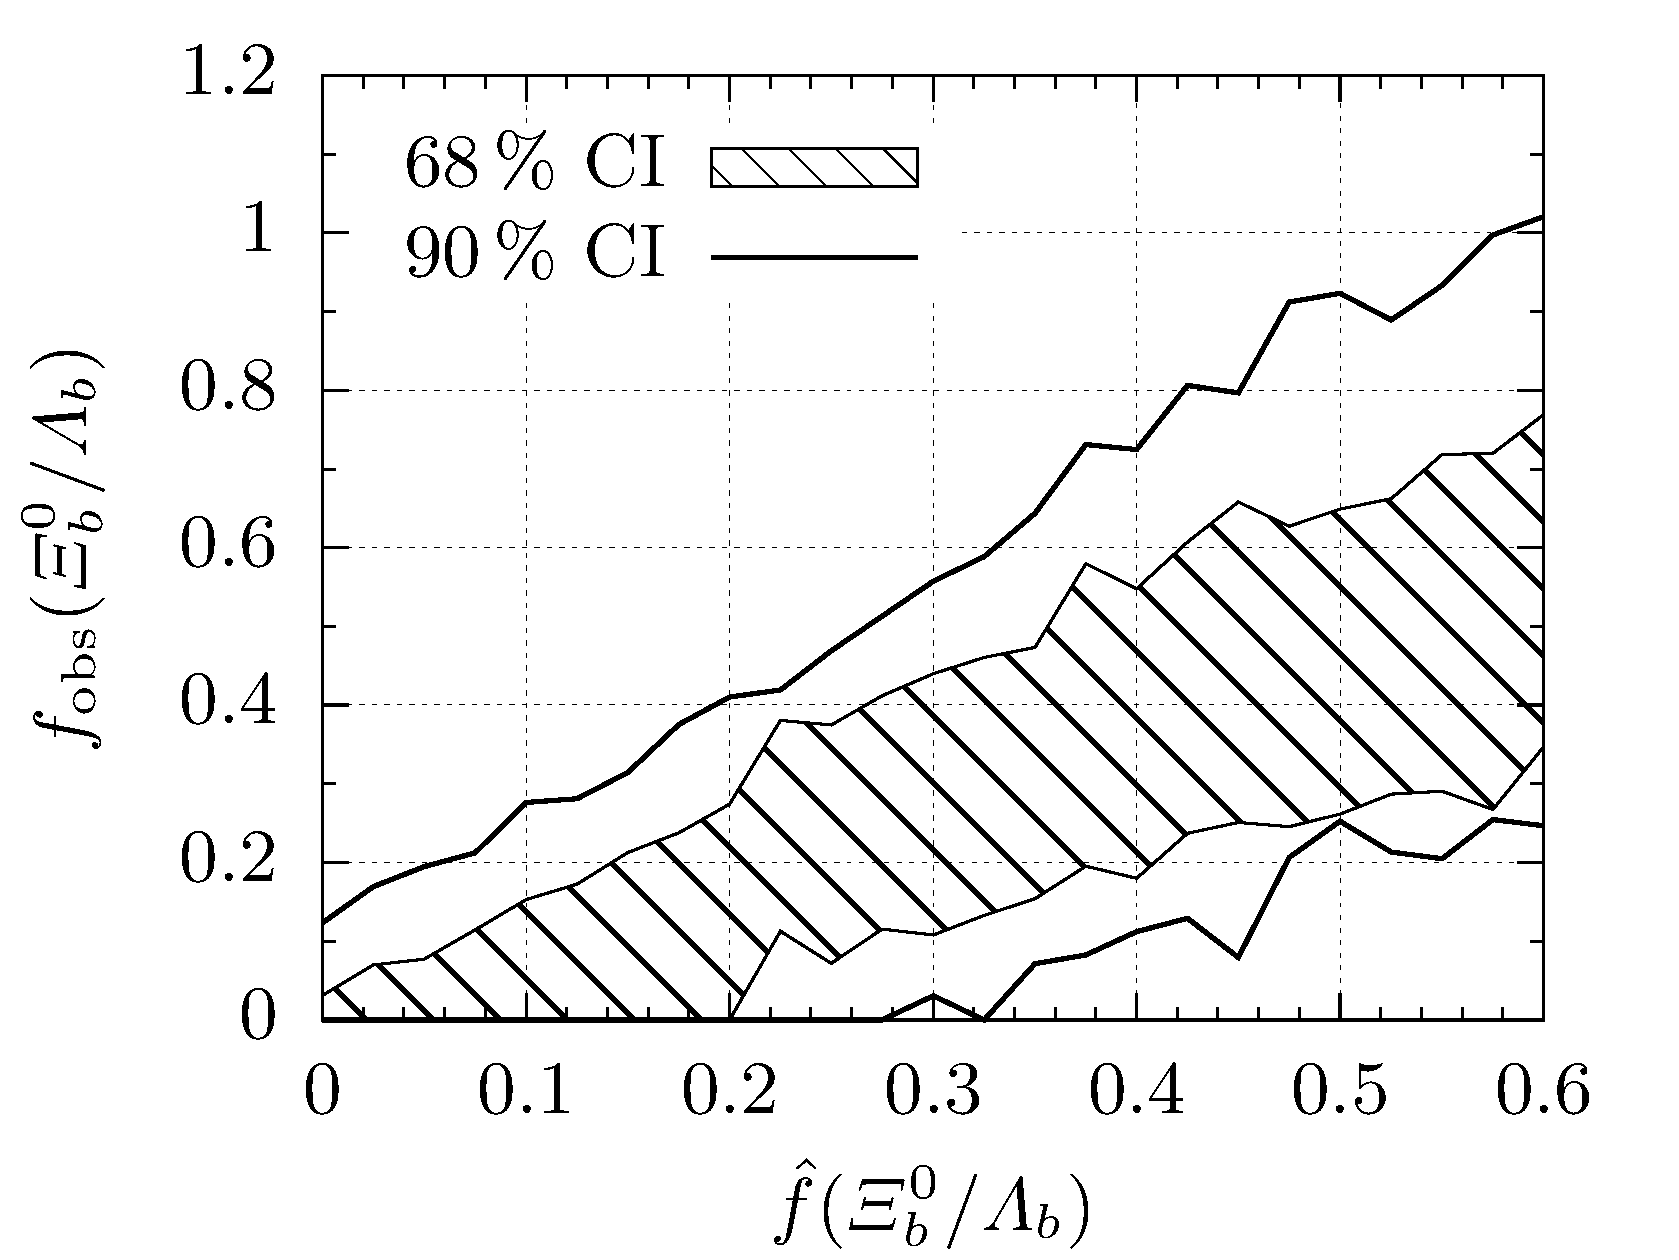
\includegraphics[scale=1.]{br/freqci_shortest.png}
    \end{subfigure}
    \begin{subfigure}{.49\textwidth}
        \centering
        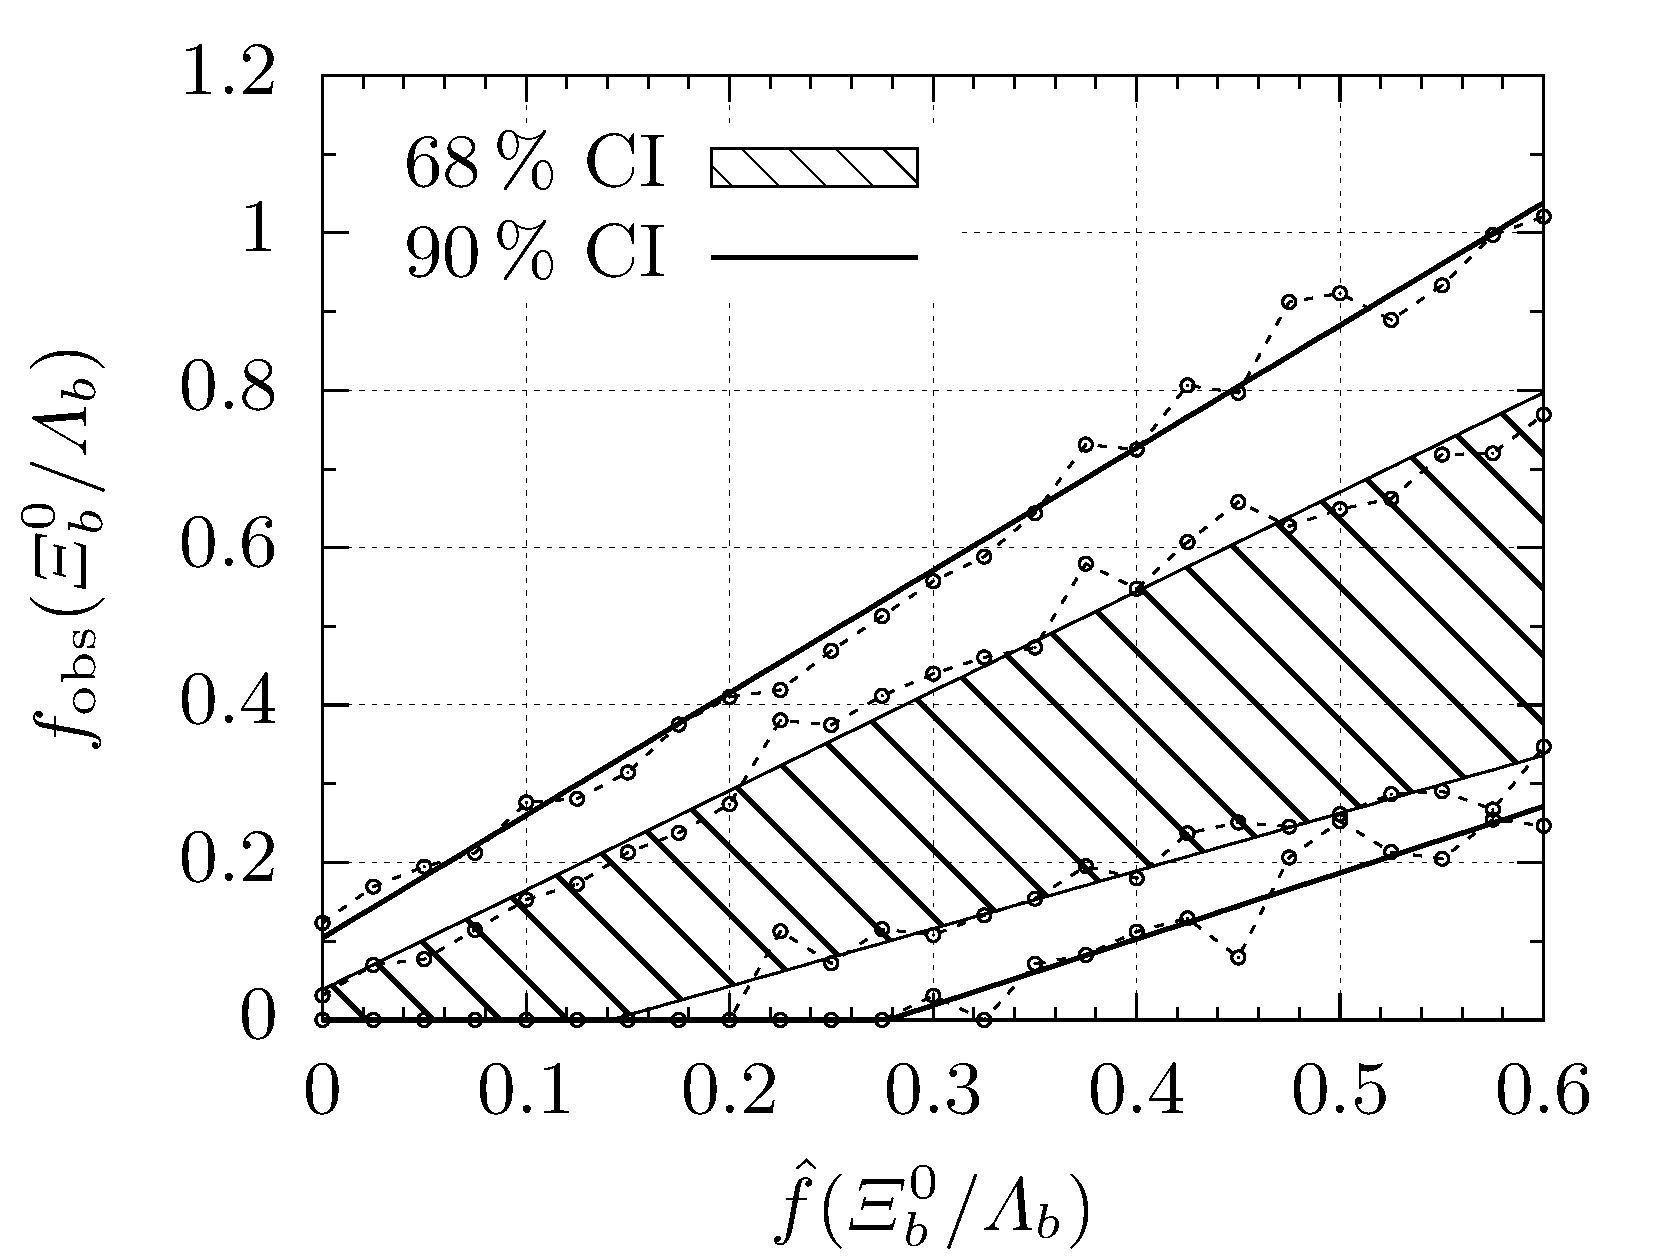
\includegraphics[scale=1.]{br/freqci-fit_shortest.png}
    \end{subfigure}
    \caption{Frequentist CIs using the \textit{shortest} method. Interval boundaries are estimated by finding the shortest intervals in $f_\text{obs}(\Xibz/\Lb)$ with a coverage of 68\,\% and 90\,\% at 25 different $\hat f(\Xibz/\Lb)$ positions. The boundaries (left) are smoothed with linear functions (right).}
    \label{fig:apdx_brxiblb_freqci_shortest}
\end{figure}

As an alternative, we also calculate CIs using Bayesian methods by converting the fitted likelihood, as shown in Fig.~\ref{fig:apdx_brxiblb_likelihood}, into an a posteriori probability density (using Bayes theorem).
This transformation involves a normalization and an assumption about the prior probability.
The latter is non-obvious and we decide to estimate intervals based on the assumption of a uniform distribution of $f(\Xibz/\Lb)$.
In Fig.~\ref{fig:apdx_brxiblb_bayesci} we show the results of integrating the \gls{pdf} when using the \textit{central} and \textit{shortest} method.
Again, 84\,\% CL and 95\,\% CL upper limits are implicitly given by the \textit{central} 68\,\% and 90\,\% interval, respectively.
A comparison of the presented methods is shown in Fig.~\ref{fig:br_xiblb_brs} and Tab.~\ref{tab:br_xiblb_brs}.

\begin{figure}[htbp]
    \centering
    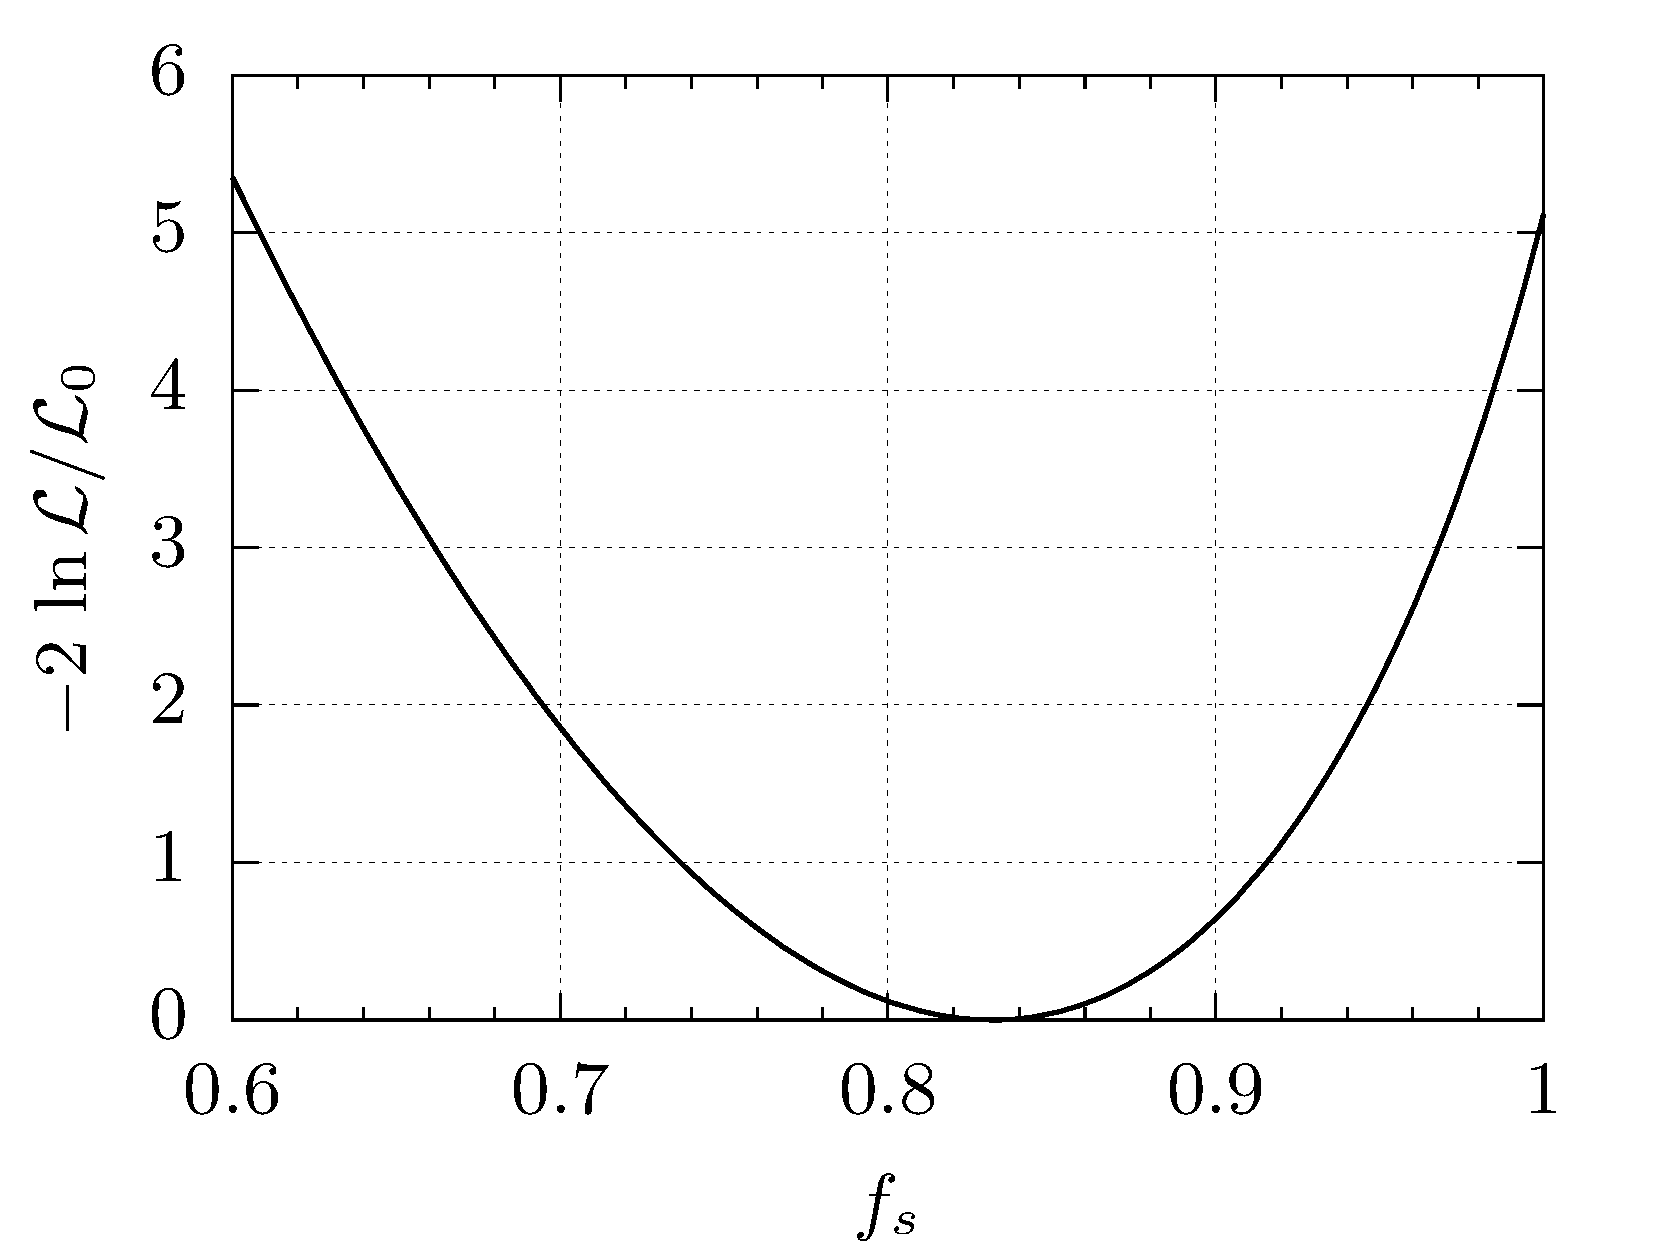
\includegraphics[scale=1.]{br/fs_profile_truex.png}
    \caption{Normalized log-likelihood ratio of $f_s$ as estimated by the fitting procedure. The normalization is chose such that intervals using the likelihood ratio method can directly be read off the $y$-axis.}
    \label{fig:apdx_brxiblb_likelihood}
\end{figure}

\begin{figure}[htbp]
    \centering
    \begin{subfigure}{.49\textwidth}
        \centering
        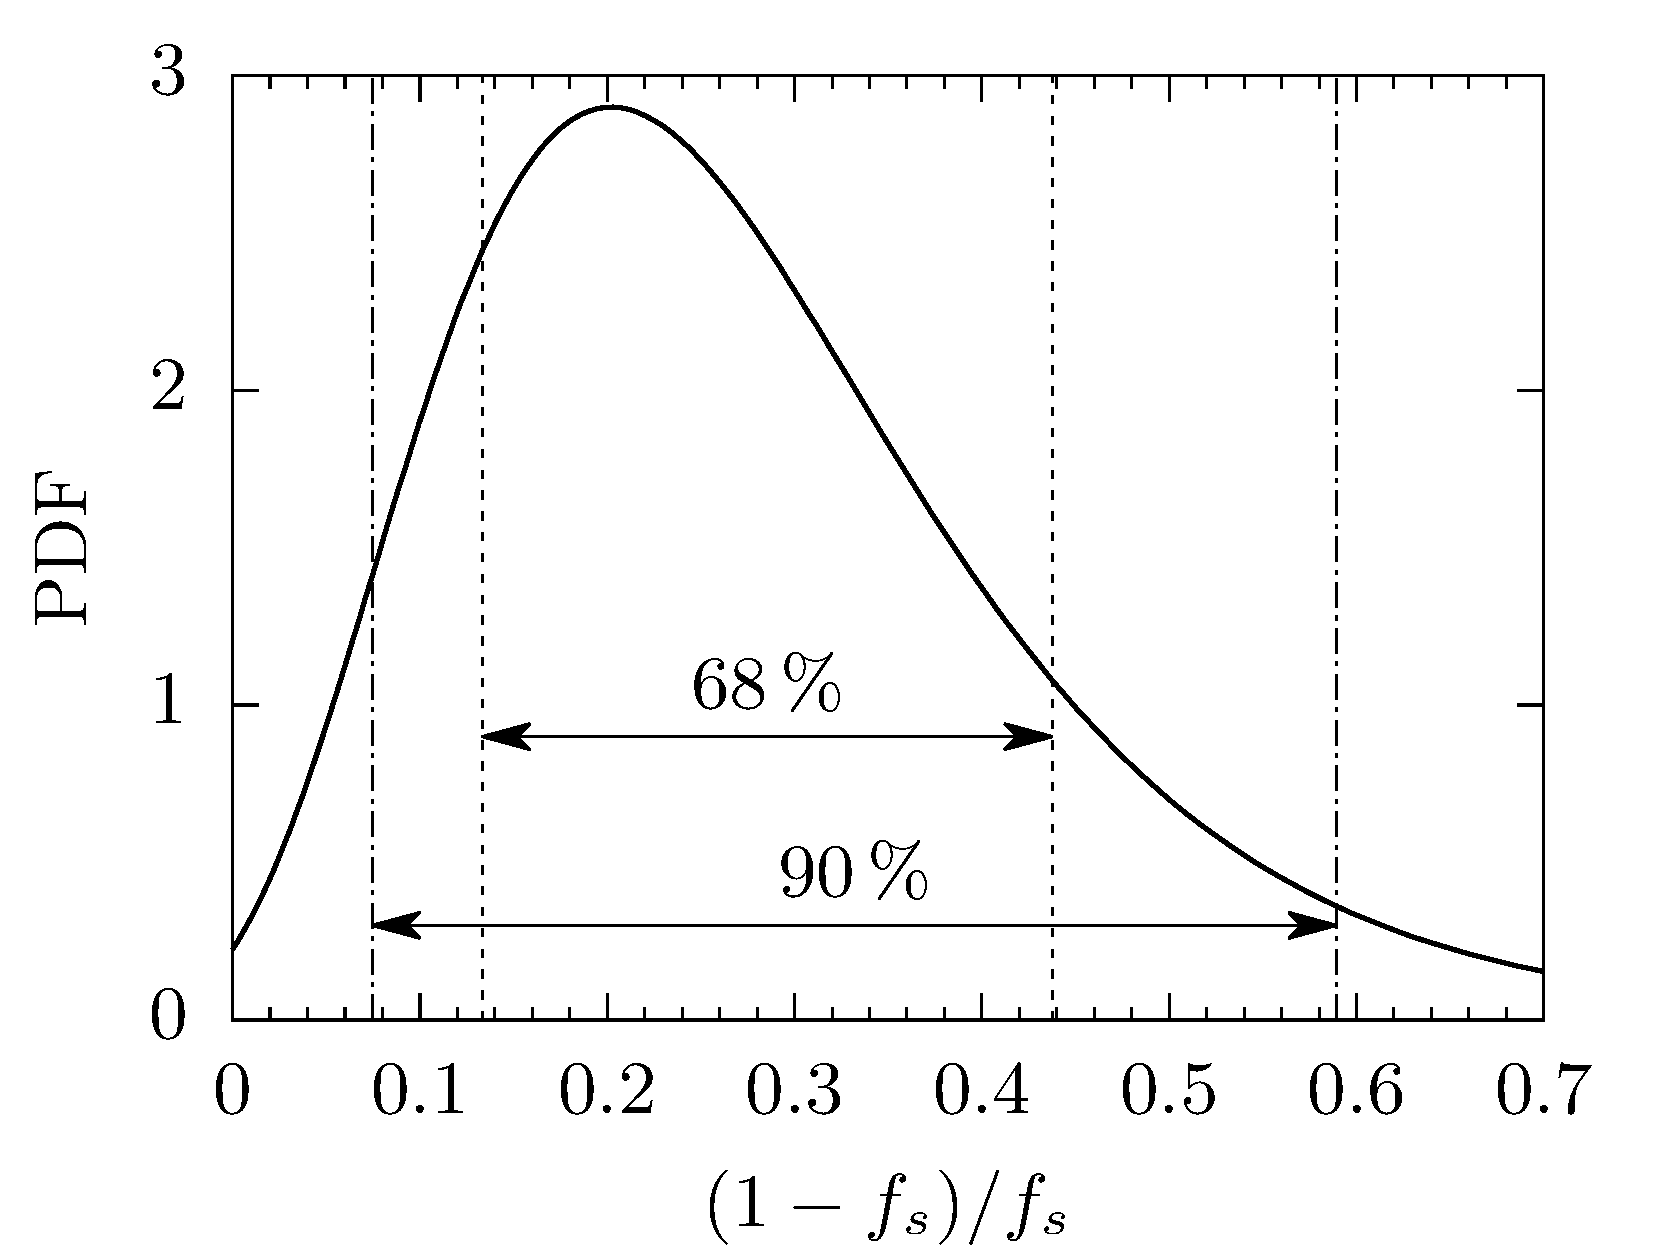
\includegraphics[scale=1.]{br/fs_profile_bayes_central.png}
        \caption{Central}
    \end{subfigure}
    \begin{subfigure}{.49\textwidth}
        \centering
        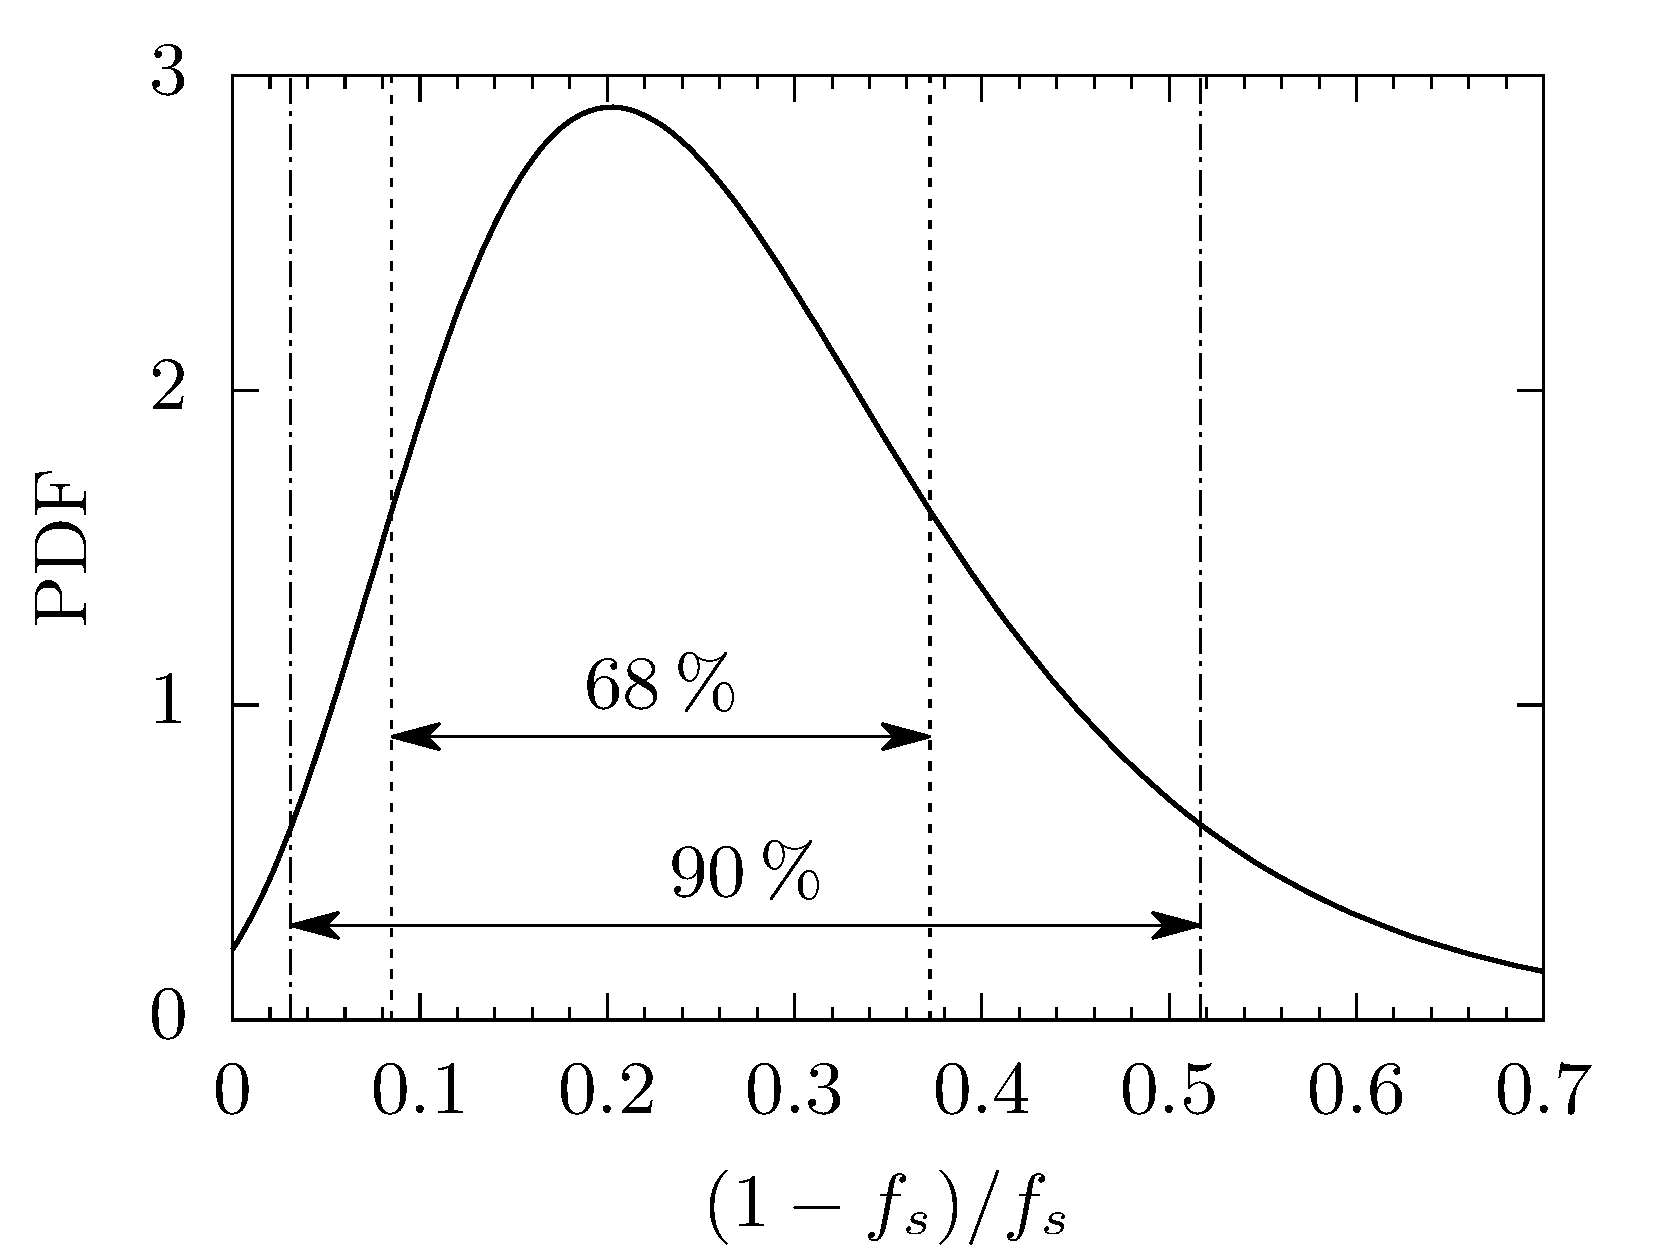
\includegraphics[scale=1.]{br/fs_profile_bayes_ep.png}
        \caption{Shortest}
    \end{subfigure}
    \caption{Bayesian CIs by integrating the normalized likelihood of $f(\Xibz/\Lb)$ as estimated by the fitting procedure, assuming a uniform distribution of the prior. On the left (right) intervals are chosen according to the \textit{central} (\textit{shortest}) method.}
    \label{fig:apdx_brxiblb_bayesci}
\end{figure}

\begin{figure}[htbp]
    \centering
    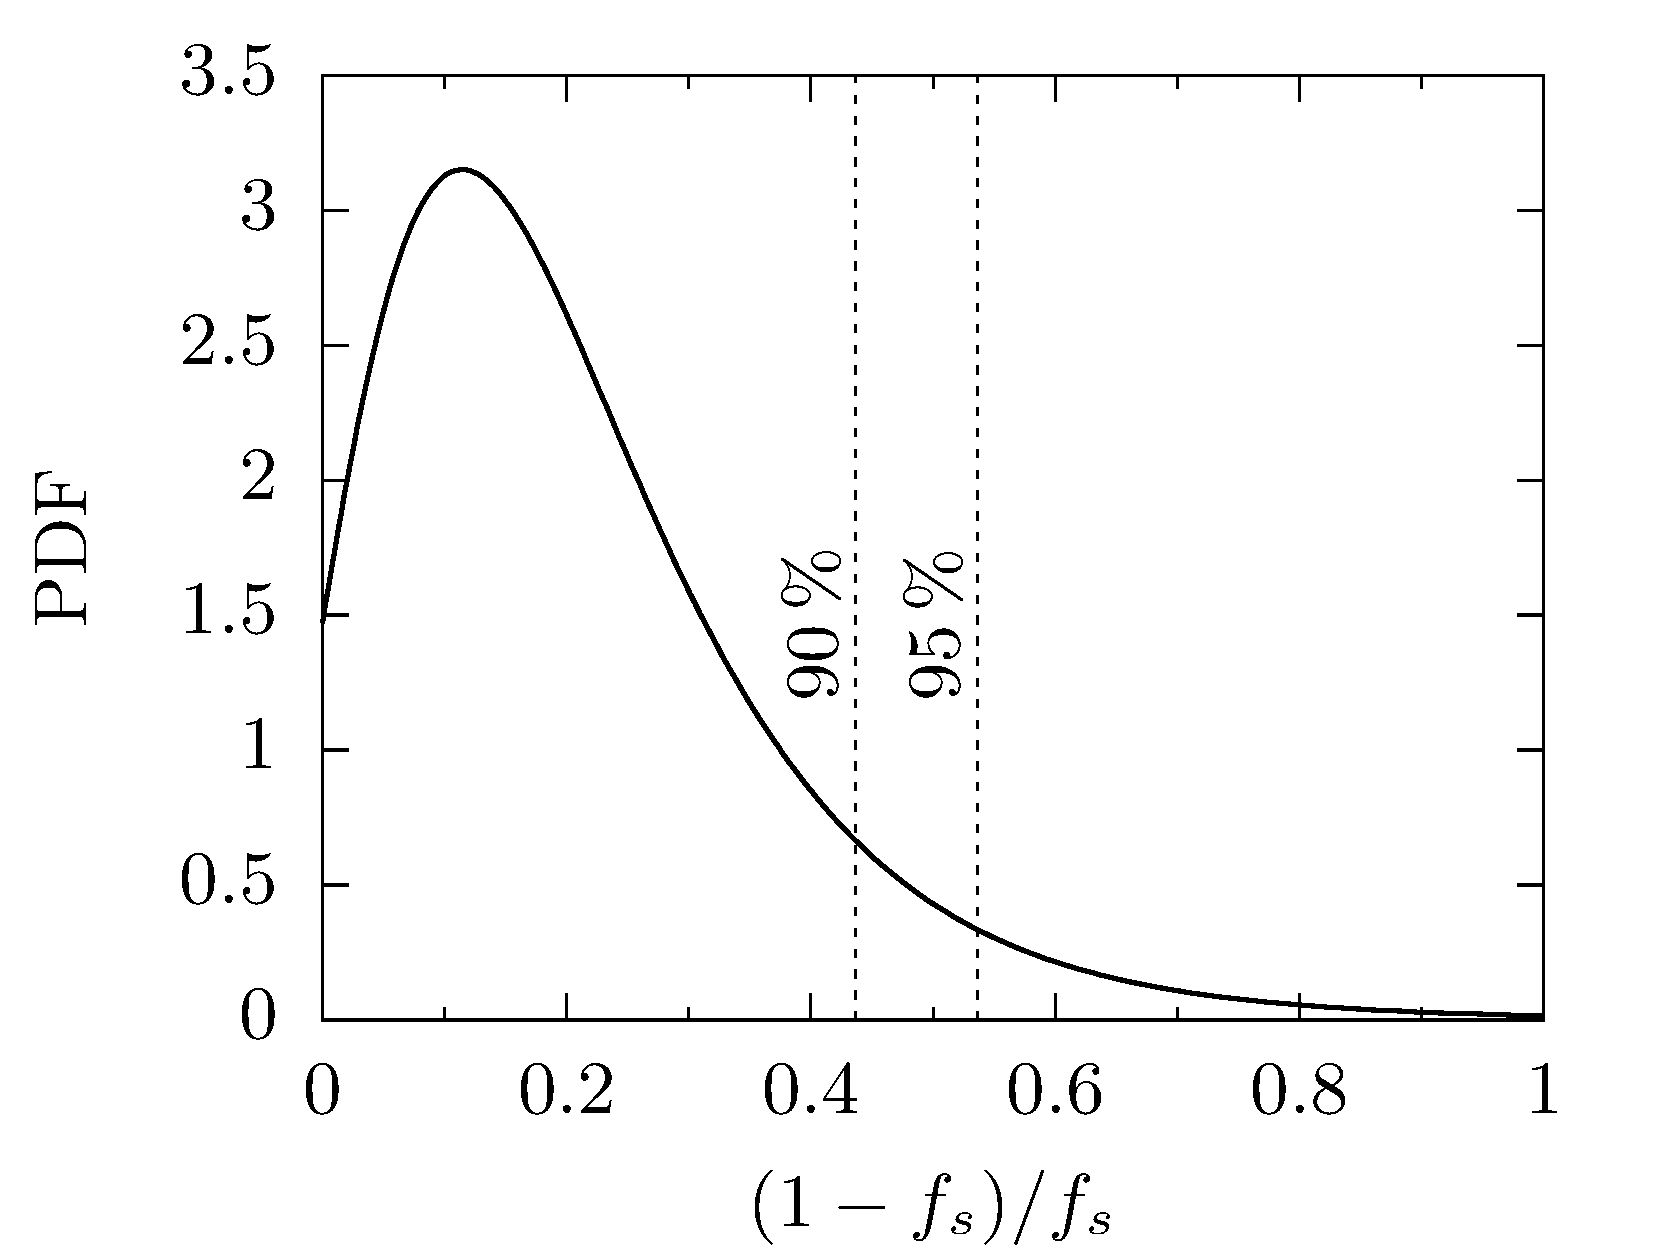
\includegraphics[scale=1.]{br/fs_profile_bayes2.png}
    \caption{Bayesian upper limits by integrating the normalized likelihood of $f(\Xibz/\Lb)$ as estimated by the fitting procedure, assuming a uniform distribution of the prior, when an additional veto against charmless \Xibz backgrounds is required.}
\end{figure}
